\chapter{Solar flare detection}

Before starting to write the main solar flare detection algorithm a first program was developed in which the location of the sun was known and we knew when a powerful solar flare had taken place.

Try algorithm knowing the location of the source, sun. Show first distribution of VTEC thtough the day (vill), then for the specific moment in time

\section{Data}

\subsection{GPS Data}

Hablar de donde salen, el fichero ti me lo ha dado manuel. El fichero ti es el resultado de "pre-procesar" los datos Raw que hay en la web de ftp://cddis.nasa.gov/.

Explicar que es cddis, como se procesan los datos, link al \cite{hernandez2009igs}, ahi esta explicado como los procesa

\subsection{The Halloween Storm}

To test this, the data used was that of the called "Hallowen Storm, in which 

Halloween storm, poner ejemplos, citar al texto, porque esta tormenta otros papers de la storm tambien, decir que usaremos el momento exacto 11.05

\subsection{Formatting}
hablar de los datos, el formato, relevant to this algorithm: mappingion, d2li, etc

\subsection{AWK}

Usaremos awk, como va, muy breve



\section{VTEC distribution}

Fisrt we wanted to obtain VTEC distribution throughout the day, to see if any spikes appeared confirming that the moment we were going to study was correct.



\subsection{Computing the VTEC}

Although the VTEC can be computed, it can be estimated using another approach.

bla bla bla justify the following equation

\begin{equation} \label{eq:1}
	\frac{d^{2}V}{dt^{2}} = \frac{d^{2}Li}{M}
\end{equation}

Where $M=\frac{1}{\cos Z}$ is the "ionospheric mapping function", given by the inverted cosine of the satellite-zenith angle that we have for each IPP. \cite{hernandez2012gnss}

Therefore, we can estimate the VTEC of an IPP by dividing two of the given fields in the data file:
\begin{equation} \label{eq:2}
	VTEC \approx \frac{d^{2}Li}{M}
\end{equation}
The Vtec...formulas...d2li/mappingio


\subsection{The solar flare}

Because the only operation that had to be performed was the previous division, a simple AWK script was used to filter out the two necessary fields from the data file (d2li and  mapping ) and print the resulting value and the time. 

\begin{lstlisting}[language=Awk, caption=process]
{
	/a/
	d2li = $21;
	mappingFunc = $43;
	vtec = d2li/mappingFunc;
	print $3 " " vtec
}
\end{lstlisting}

\begin{lstlisting}[language=Bash, caption=Bash script to execute the procedures]
#!/bin/bash
tiDataFile="../data/ti.2003.301.10h30m-11h30m.gz"
filename=vtecDistribution

zcat "$tiDataFile" | gawk -f previewVTECDistribution.awk > vtecValues
gnuplot -e "set terminal png; set output 'vtecDistribution.png'; set title 'VTEC Distribution'; set xlabel 'Time of the day (hours)'; set ylabel 'VTEC'; set grid; plot \"vtecValues\" using 1:2 with point"
rm vtecValues
\end{lstlisting}
\clearpage

\subsection{Results}

The bash script executes the AWK process with the data as the input and outputs n rows with two columns: the time of the day and the calculated VTEC, and plots the results using Gnuplot.
This can be seen in figure \ref{fig:vtecDistribution}, we're we can see how the VTEC value evolves throught the day. Visually, a spike can be seen between 11 and 11.2 hours.

\begin{figure}[!htb]
	\begin{subfigure}[b]{0.5\textwidth}
		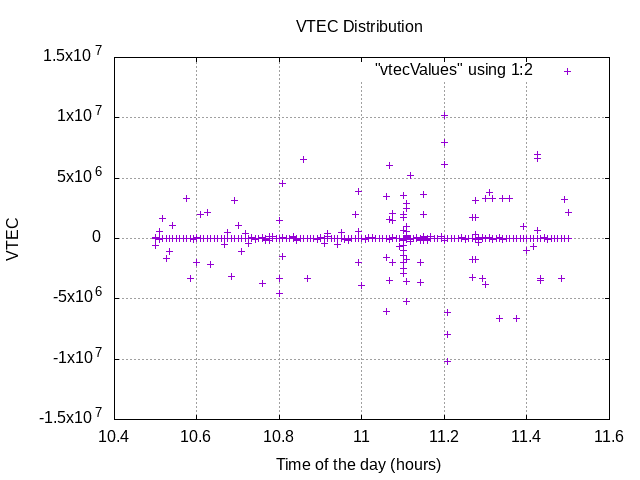
\includegraphics[width=\linewidth]{images/ch4/vtecDistributionGeneral.png}
		\caption{All IPPs}
	\end{subfigure}
	\hfill
	\begin{subfigure}[b]{0.5\textwidth}
		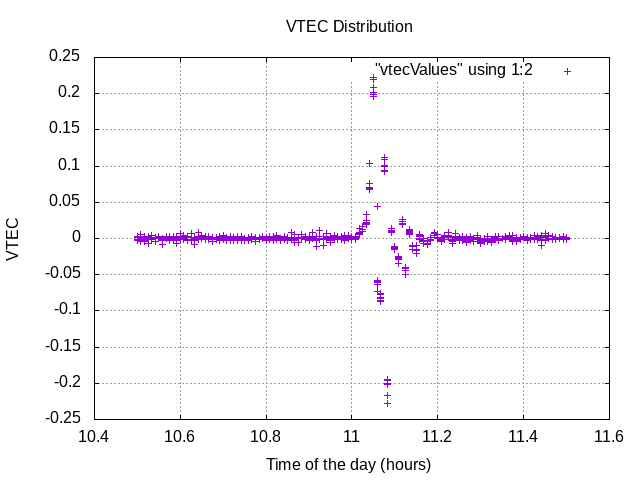
\includegraphics[width=\linewidth]{images/ch4/vtecDistributionVill.png}
		\caption{Vill}
	\end{subfigure}
	\caption{VTEC distribution throughout the day for all IPPS (a) and for IPPs that have Vill as the receiver (b)}
	\label{fig:vtecDistribution}
\end{figure}

To see the event more clearly, though, we can focus on one specific receiver (which will still yield multiple IPPs, as the receiver works with different satellites). For the particular case of the Vill station, which at that time of the day would be under the sun, we obtain the following plot, in which the spike can be seen more clearly. As mentioned before, the flare took place at 11.05.


primer paso, ver datos de un IPP
Awk prepocesado de datos
fortran
gnu plot para empezar a ver



\section{Algorithm, here or new chapter?}

\subsection{VTEC value}

\subsection{Solar-zenith angle}









After that, talk about proposals for the main algorithm

explicar que vamos a hacer – IPPs, hill climbing y buscar si una vez en un pico, hay relacion lineal entre VTEC I coseno. En lugar de eso, subir mirando






\section{Pseudocode}

\begin{algorithm}
	\caption{My algorithm}\label{euclid}
	\begin{algorithmic}[1]
		\Procedure{MyProcedure}{}
		\State $\textit{stringlen} \gets \text{length of }\textit{string}$
		\State $i \gets \textit{patlen}$
		\BState \emph{top}:
		\If {$i > \textit{stringlen}$} \Return false
		\EndIf
		\State $j \gets \textit{patlen}$
		\BState \emph{loop}:
		\If {$\textit{string}(i) = \textit{path}(j)$}
		\State $j \gets j-1$.
		\State $i \gets i-1$.
		\State \textbf{goto} \emph{loop}.
		\State \textbf{close};
		\EndIf
		\State $i \gets i+\max(\textit{delta}_1(\textit{string}(i)),\textit{delta}_2(j))$.
		\State \textbf{goto} \emph{top}.
		\EndProcedure
	\end{algorithmic}
\end{algorithm}

\begin{lstlisting}[language=Python, caption=Python example]
import numpy as np

def incmatrix(genl1,genl2):
	m = len(genl1)
	n = len(genl2)
	M = None #to become the incidence matrix
	VT = np.zeros((n*m,1), int)  #dummy variable
	
	#compute the bitwise xor matrix
	M1 = bitxormatrix(genl1)
	M2 = np.triu(bitxormatrix(genl2),1) 
	
	for i in range(m-1):
	for j in range(i+1, m):
	[r,c] = np.where(M2 == M1[i,j])
	for k in range(len(r)):
	VT[(i)*n + r[k]] = 1;
	VT[(i)*n + c[k]] = 1;
	VT[(j)*n + r[k]] = 1;
	VT[(j)*n + c[k]] = 1;
	
	if M is None:
	M = np.copy(VT)
	else:
	M = np.concatenate((M, VT), 1)
	
	VT = np.zeros((n*m,1), int)
	
	return M
\end{lstlisting}

